\section{Gestione degli utenti}
Per gestire al meglio la procedura di autenticazione dell'applicazione, la
registrazione e le preferenze dei singoli utenti, si è scelto di utilizzare
Firebase, servizio di database basato sul cloud appartenente a Google.

\subsection{Firebase}
Firebase è un ottimo servizio di backend che rende disponibili, tramite API,
numerosi servizi tra cui lo storage dei dati, l'autenticazione, notifiche push e
molto altro. Una delle caratteristiche più utili di questo servizio è la
capacità di sincronizzazione dei dati oltre che di storage: le informazioni
vengono infatti aggiornate pressochè all'istante, a patto che l'app web o mobile
sia collegata alla rete. Inoltre sono disponibili numerose librerie client che
rendono ancora più semplice l'integrazione con il proprio prodotto software.
Anche la sicurezza ha un aspetto rilevante, in quanto i dati immagazzinati sono
replicati e sottoposti continuamente a backup e la comunicazione con il client
avviene in modalità crittografata tramite SSL con certificati a 2048 bit.
Esistono tre piani tariffari per utilizzare Firebase. Il primo, gratuito, è
chiamato Spark e comprende i servizi base, tra cui l'autenticazione, fino a 100
connessioni simultanee, 1 GB totale di spazio per i dati e 5 GB per lo storage
di immagini e file. Il secondo è il Flame Plan nel quale aumentano i limiti (50
GB per lo storage e fino a 2,5 GB per i dati) al costo di 25\$ al mese.
L'ultimo è il Blaze Plan nel quale ogni servizio possiede un costo unitario
relativamente basso e funziona con una politica \textit{pay as you go}. Per le
esigenze del progetto il primo piano (Spark) era più che sufficiente.

\subsection{Schermata di avvio, tipologia di Utente e pagina Profilo}
Nella schermata d'avvio (figura \ref{login}) l'utente può scegliere di accedere
all'applicazione in tre modi diversi: tramite accesso standard (utente
standard), tramite il pulsante \textit{Accedi con Google} (utente Google) o
tramite accesso anonimo. A seconda della tipologia, le pagine accessibili
cambiano, così come i servizi disponibili.
\begin{figure}[h!]
    \centering
    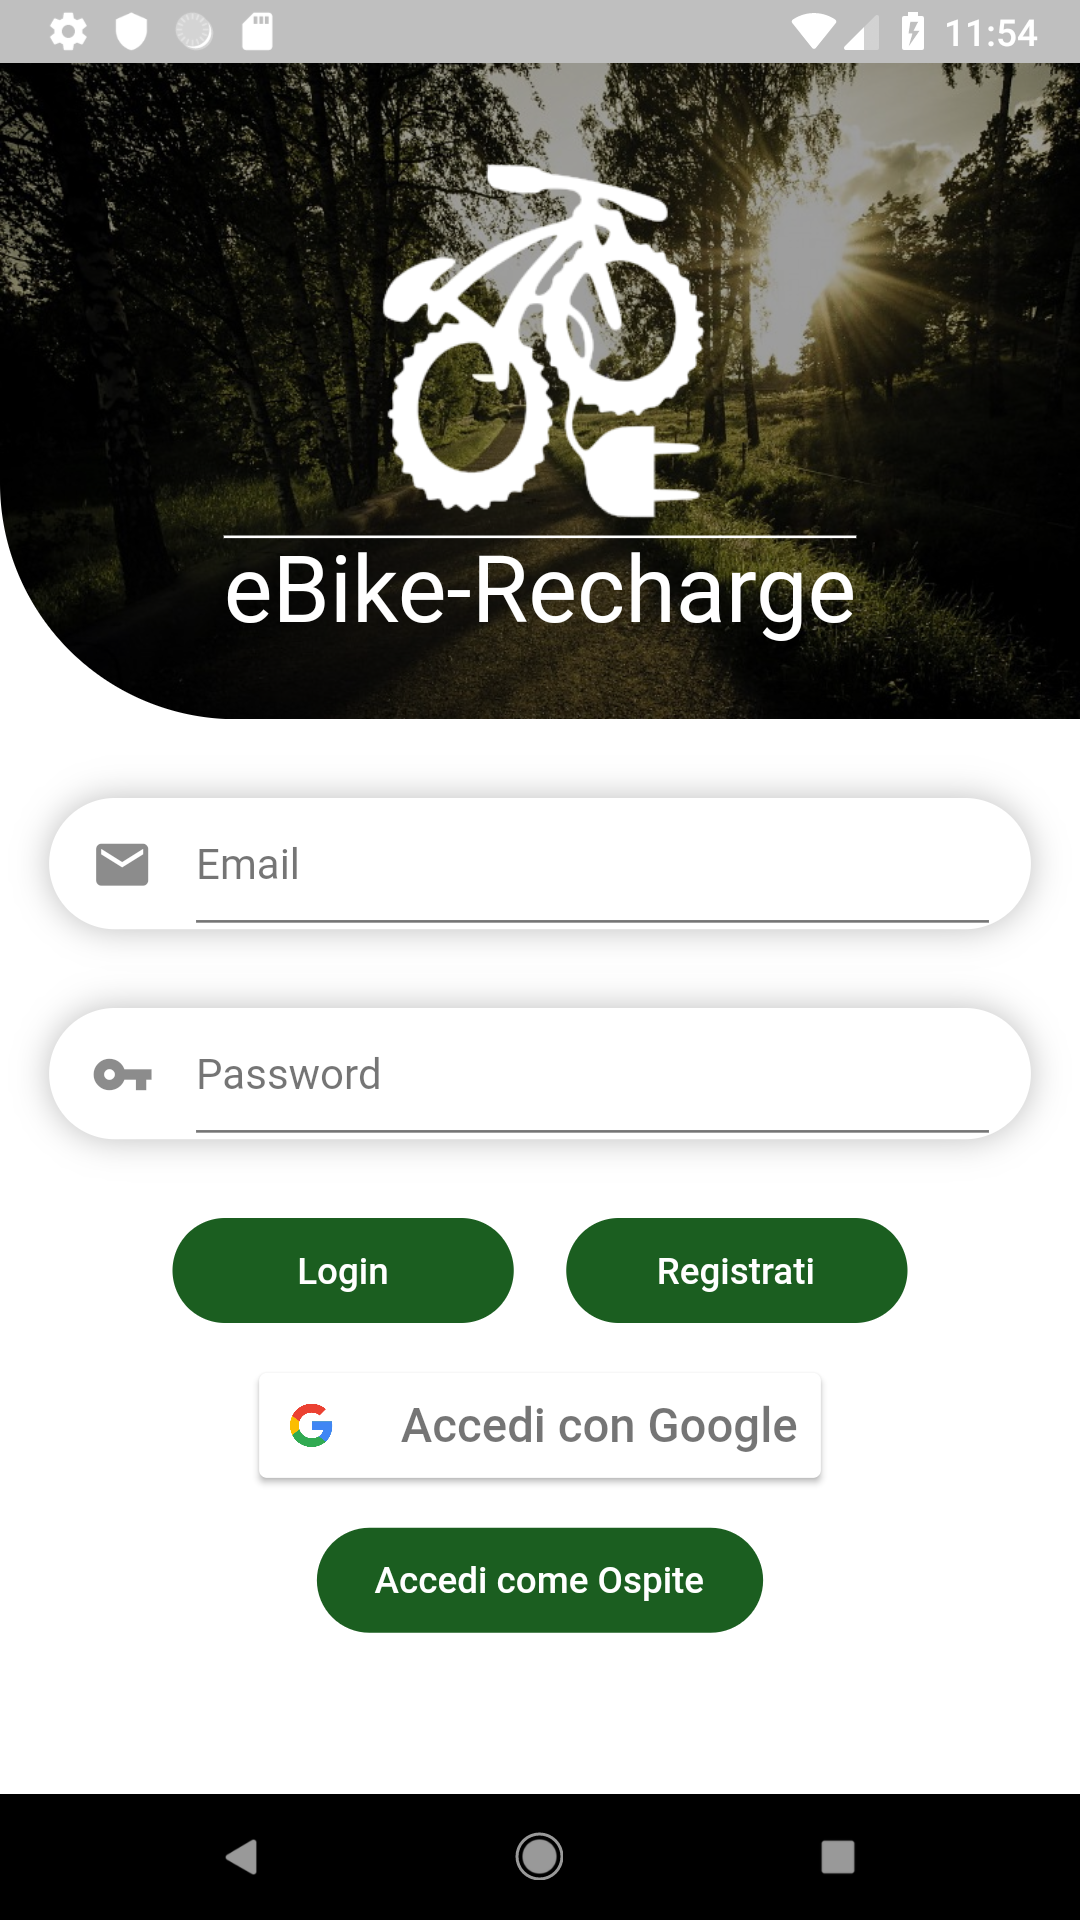
\includegraphics[scale=0.15]{Login.png}
    \caption{Schermata d'avvio}
    \label{login}
\end{figure}
Se l'utente è gia registrato in modo standard, può inserire la propria mail
(usata come username) e la propria password. Se i dati forniti combaciano con
quelli presenti nel database degli utenti si fa accesso alla pagina della mappa
che verrà descritta in un prossimo capitolo. Se invece non c'è corrispondenza
con un utente già registrato viene mostrato a video un messaggio di errore che
spiega cosa è successo. \newline
Si può anche fare accesso all'applicazione utilizzando i servizi Google che
permettono di autenticarsi mediante gmail, con il proprio
account Google. In questo caso si apre una nuova finestra (codificata grazie ad
una API) che mostra gli account gmail utilizzati sul proprio dispositivo e dopo
aver inserito la password si fa accesso alla pagina della mappa. In particolare
la grande differenza tra i due tipi di accesso appena citati consiste nella
pagina profilo utente presente nell'applicazione. Questa è accessibile premendo
l'icona \textit{Profilo} presente nella TabBar in basso sullo schermo. In alto
viene indicata la mail dell'utente (sia che essa faccia parte di gmail, sia che appartenga
ad un altro dominio), e vengono poi mostrati diversi pulsanti ognuno con una
specifica funzione. Quelli con scritto "Tipo Mappa", "Stazioni Aggiunte" e "Log
Out" sono presenti in entrambe le versioni e permettono rispettivamente di
cambiare il tipo mappa ed esaminare le stazioni aggiunte dall'utente che sta
usando l'applicazione (entrambe queste funzionalità sono discusse nel capitolo
riguardante la mappa), e di uscire dal particolare account in uso e tornare alla
pagina di Login. Se l'utente è di tipo standard, è presente un ulteriore
pulsante con scritto "Cambia Password": esso permette grazie a un'API di
Firebase di cambiare la propria password nel caso in cui si sia dimenticata.

\subsection{Registrazione}
Nel caso in cui l'utente effettui il primo accesso oppure desideri creare un
nuovo utente, deve solo premere il pulsante "Registrati", per andare nella
pagina di registrazione. Essa mostra tre campi di testo dove bisogna inserire la
propria mail, la password, e confermare quest'ultima reinserendo la stessa
password. Vengono effettuati dei controlli di integrità dei dati (così come
nella pagina di login): infatti tramite una \textit{regular expression} si
controlla che la mail inserita possa esistere, cioè presenti almeno una
lettera seguita da una \MVAt, almeno due ulteriori lettere, un punto e almeno un'altra
lettera. Inoltre la password deve possedere almeno sei caratteri e la sua
conferma deve ovviamente combaciare con quella inserita prima. Se tutto è
corretto l'utente può premere il tasto "Registrati", venendo quindi portato alla
pagina della mappa e creando così un nuovo account standard. \newline
Se l'utente non effettua il logout nella pagina Profilo, ogni volta che accede
all'applicazione sarà subito portato alla pagina della mappa senza dover passare
dalla pagina di login, questo accade perchè grazie a Firebase si tiene traccia
dello stato della sessione del particolare account.

\begin{figure}[h!]
    \centering
    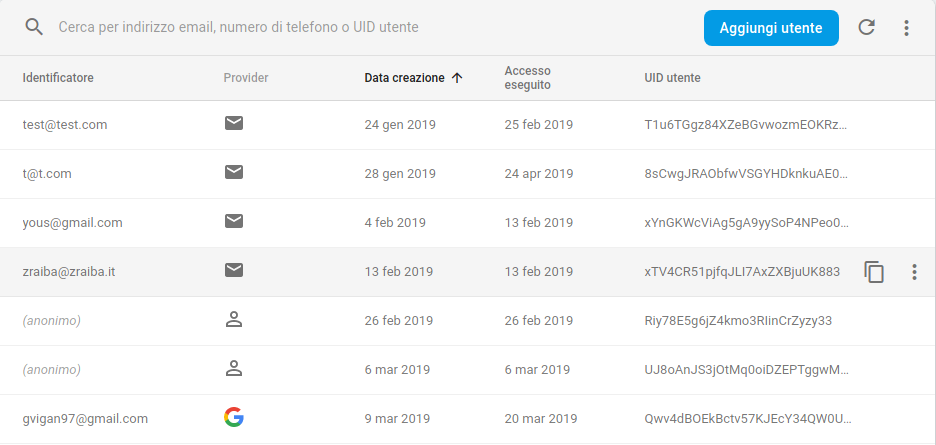
\includegraphics[width=13.5cm]{Authentication.png}
    \caption{La sezione Authentication di Firebase}
    \label{authentication}
\end{figure}

\subsection{Utente anonimo}
Nella pagina di login è anche possibile premere il tasto "Accedi come Ospite" in
fondo allo schermo, e questo pulsante permette di accedere all'applicazione
senza dover registrare nessun account. La struttura dell'app cambia radicalmente
se si esegue questo tipo di accesso. Innanzitutto sono presenti solo due pagine
accessibili (e non più tre come nel caso standard e Google) e consistono in una
pagina mappa con funzionalità estremamente ridotte e una pagina di Upgrade nella
quale si mostra all'utente i posibili privilegi raggiungibili al momento di
un'autenticazione registrata. Nella sezione \textit{Authentication} del servizo
online di Firebase (figura \ref{authentication}) è possibile prendere visione di tutti gli utenti che hanno
fatto accesso all'applicazione almeno una volta indicando la data di ultima
visita, la data di creazione e l'id dell'utente. Inoltre ne viene indicato anche
il tipo, sia esso standard, Google o un utente anonimo.

\subsection{Codifica}
